\documentclass[A4paper, 12pt]{article}
\usepackage{fancyhdr}
\usepackage{graphicx}
\usepackage{booktabs}
\usepackage{pdfpages}
\pagestyle{fancy}
\lhead{Vulcano 2.0: A New Beginning}
\rhead{v2.02}
\cfoot{\thepage}
\renewcommand{\headrulewidth}{0.4pt}
\renewcommand{\footrulewidth}{0.4pt}
\begin{document}
\title{Vulcano 2.0: A New Beginning}
\author{The Vulcano Team}
\date{\today}
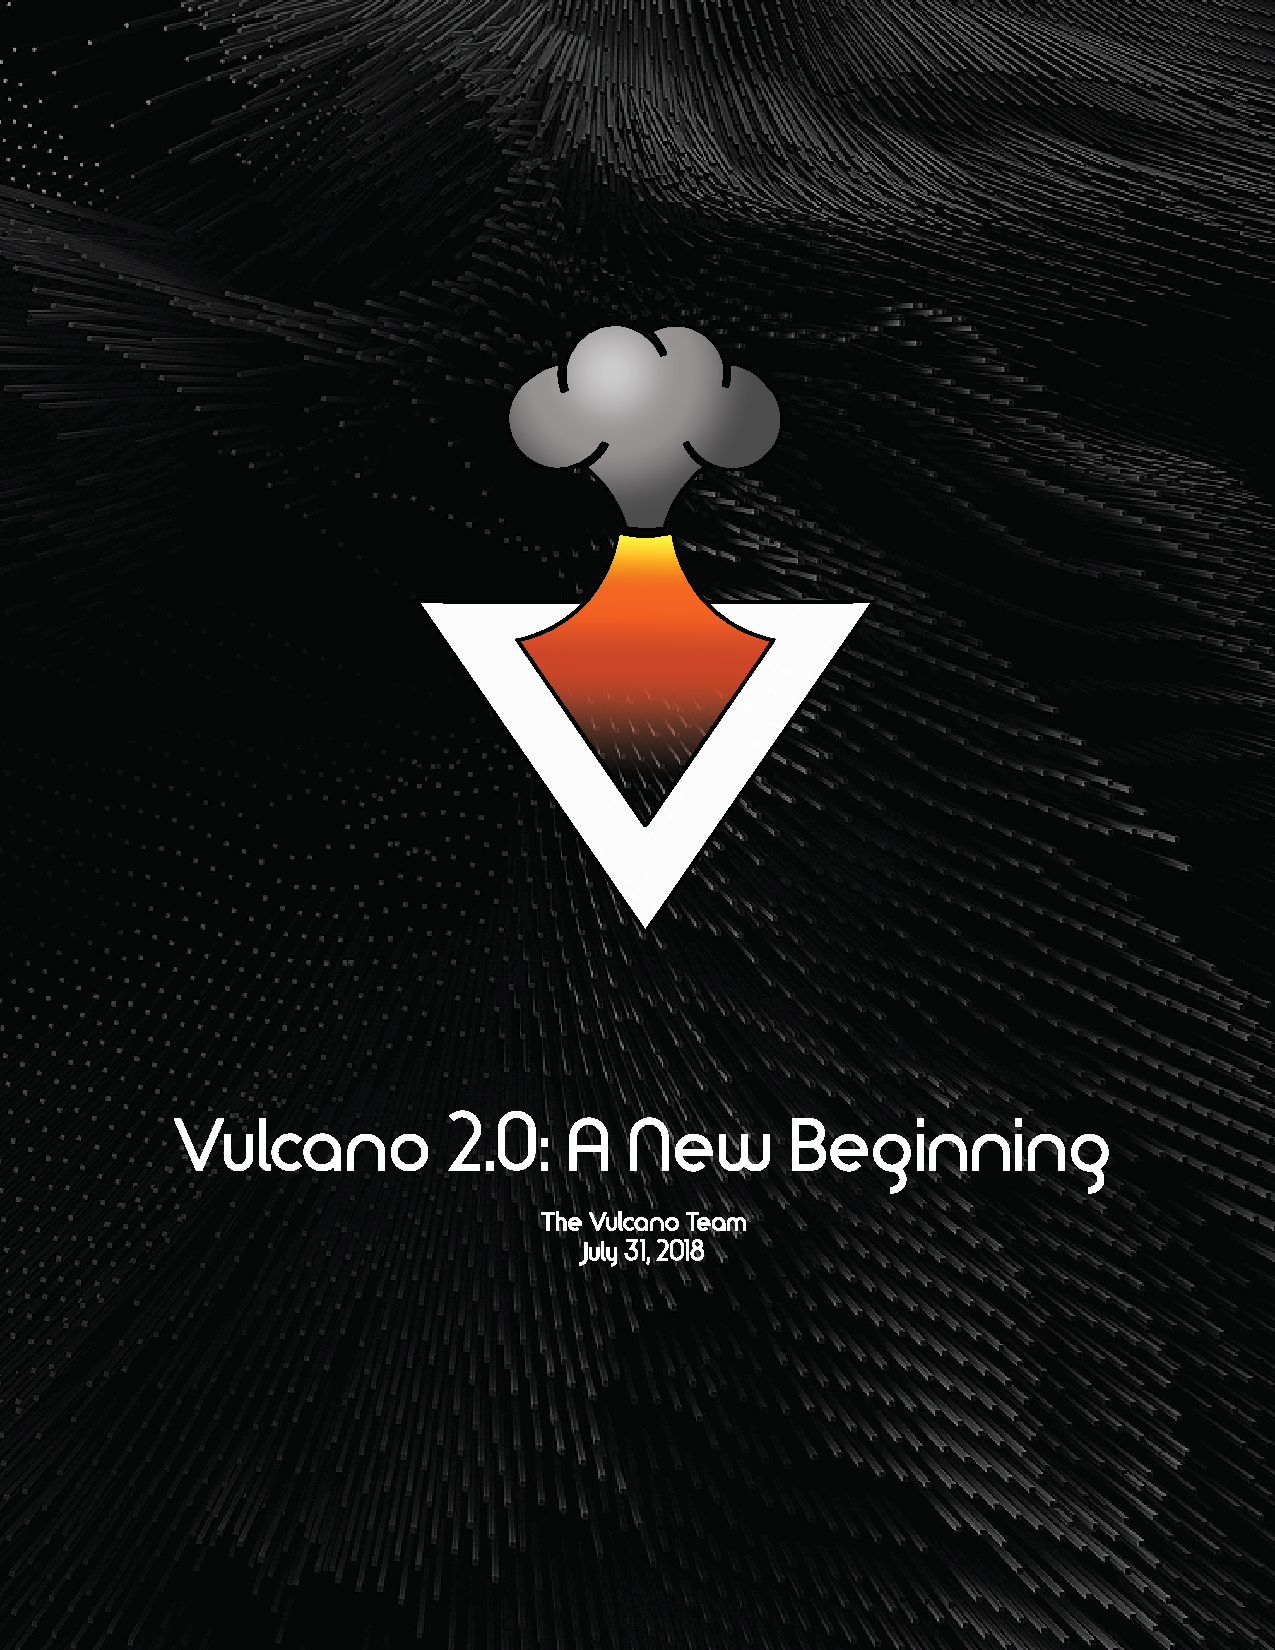
\includepdf[pages=1]{COVER.pdf}
\newpage
\tableofcontents
\newpage
\section{Introduction}

Vulcano (ticker: VULC) is a community-oriented coin originally created at the end of 2017 by a now completely absent development team. Initially, it was conceived as only a "high staking coin" with an annual return of 950\%. However, due to several errors on the part of the initial development team, the actual rate was closer to 320,000\%. This passed unnoticed until a member of the community calculated this effective rate by examining the blockchain from the Genesis Block\footnote{Brink, Jason - "Vulcano(\$VULC): Why Researching Altcoins is so Important"}. Once this fundamental weakness was exposed, the new Vulcano team, comprised of members of the community, came together to both salvage the Vulcano project on both a technical and philosophical level through a complete rebuild and the development of a real use case. This whitepaper lays out a strategy for a total upgrade of Vulcano and a relaunch of the newly upgraded coin as a means to fund geothermal exploration and research.

Rather than simply fixing the percentage rate problem with Vulcano, we have elected to completely upgrade the coin to a new code base. In order to best modernize the Vulcano Core, the Vulcano team has decided upon Bulwark as a code base. Bulwark is built upon PIVX, which itself is built upon the popular DASH cryptocurrency. This critical decision will give us the ability to implement masternode functionality, governance, and eventually allow the integration of hardware nodes to support the Vulcano ecosystem. In doing so, we will create a more truly decentralized system of governance and coin staking and network security.

This paper will also lay out the future plans for the legitimization of Vulcano through the creation of the Vulcano Foundation, a planned 501(c)3 Nonprofit entity based in the United States which will allow Vulcano to grow into its own in a mature fashion and to begin to connect and enter into negotiations with the rest of the business world. This is especially important as the long-term use case of Vulcano calls for the acquisition of a portfolio of intellectual property through the research mechanism explained below. Through the creation of a portfolio of intellectual property through the funding of research at universities and research institutions around the globe. The Vulcano Foundation would enable us to best leverage this intellectual property. This is an absolutely critical step which will allow the decentralized Vulcano project to interact and connect with the centralized worlds of business and academia. 

This paper will also lay out the planned percentages of governance fees which will go directly to funding geothermal research in order to both advance the science and gain intellectual property to bring more funding to the Vulcano Foundation for future developments and to provide funding for additional grants. 

What you will not find in this paper is wild and unsubstantiated promises about the future of the Vulcano blockchain. Vulcano strives for innovation and growth without making promises that cannot be delivered upon – instead we will dedicate our efforts to research and advancing technological development. All blockchain technology mentioned in this paper has already been demonstrated and will be activated in due course. We believe that it is time for the cryptocurrency communities to begin acting in a way that is consistent with the business potential they bring to the table, and that wild claims about blockchain technology are not needed to build a business case for the use of existing technology. Developers, team leads, and the communities themselves must understand that in order to be accepted by the broader business and academic communities, we must be willing to play by their rules to a certain degree and make effective use of what we have before advancing ideas about unproven blockchain technology before it has been developed, tested, or planned out. While there may be advances in blockchain technology itself for Vulcano in the future, its release will not come with months of fanfare and marketing, but will only be spoken about once it has already been developed. We believe that this method of "submarine" development is best for the currency because it limits speculative investing and allows for the building of a stable foundation for the platform in the future. 

It is our goal to turn Vulcano into one of the premier sources of funds for sustainability research in the future and to eventually build a business ecosystem around this technology.


\section{Acknowledgements}
Vulcano would not have been possible without the prior works of the respective Bitcoin, Peercoin, Blackcoin, Talkcoin, Dash, PIVX, and most importantly, Bulwark teams. As the new incarnation of Vulcano is a modified fork of Bulwark, several sections have been borrowed directly from their whitepaper for functionalities which we will be including but which will not be modified from the existing code base. We, the Vulcano Team, felt it would be more transparent to include these sections as they existing in the Bulwark paper rather than rewriting them and pretending they are completely original content. While it is important that we, as a community, develop solid use cases and business structures which work for the broader world, the open source ethos behind cryptocurrency must be protected and maintained going into the future. Humanity, as a whole, benefits from the sharing of the information and we are proud to be contributing to this growing body of knowledge. It is in this same spirit that we will offer the technologies developed with funding through the Vulcano Foundation to nations which contribute to the Vulcano ecosystem. 

\section{A Brief Introduction to Cryptocurrencies}
While proposals for distributed ledger technology stretch back into the late 1980s, it was not until the release of a paper on an obscure cryptography bulletin board of a paper entitled, Bitcoin: A Peer-to-Peer Electronic Cash System by a writer under the pseudonym of Satoshi Nakamoto that a true blockchain was born. A blockchain works by timestamping transactions sequentially and locking them into "blocks" which are validated by various methods so that they cannot be tampered with. Bitcoin and many other cryptocurrencies operate on the basis of "Proof-of-Work", which means that they use computational power as the resource of scarcity within their network.
 
However, as Vulcano is focused on sustainability and research in the energy field, such a non-sustainable method is antithetical to our efforts to increase sustainability. Therefore, we have elected to operate on a "proof-of-stake" basis, where the resource of scarcity in the network is the tokens themselves. Additionally, with the launch of the upgraded Vulcano released 30 days following the posting of this whitepaper, we will also have masternodes, which are a somewhat more advanced version of the Proof-of-Stake method in which computers around the world maintain the network but also bear some simple computational load for the purpose. As of right now, this computational load is scarcely bigger than the operation of a simple staking wallet, but we would like to use this network in the future for distributed computing for the renewable energy industry for the operation of computational chemistry and physics problems. This is an important addition to the long-term plan for Vulcano, as the geophysics and geothermal departments at research universities are typically not as well funded as other more glamourous fields, and therefore have a harder time getting cycle time on the large computers to run their simulations. 

Additionally, from a consumer perspective, with a 90 second block time, masternode consensus and transaction locking, a controlled and stabilized emissions schedule, and eco-friendly staking, Vulcano aspires to be a truly fast and functional cryptocurrency that makes a real impact on the world but is also a strong option for consumers and cryptocurrency enthusiasts. 

\section{The New Vulcano}
\subsection{Specifics of the New Vulcano Blockchain}

\begin{table}[h]
\centering
\begin{tabular}{@{}ll@{}}
\toprule
Ticker & VULC \\ \midrule
Algorithm & NIST5 \\
RPC Port & 52541 \\
P2P Port & 52543 \\
Block Spacing & 90 Seconds \\
Difficulty Algorithm & Dark Gravity Wave v3.0 \\
Block Size & 1MB \\
Mined/Minted Maturity & 67 Blocks ($\sim$100 Minutes) \\
Confirmation & 6 Blocks ($\sim$9 Minutes) \\
Circulation (1 Year) & 246,194,250 \\
Circulation (5 Years) & 421,126,225 \\
PoW Period & nHeight ≤ 60 \\
PoS Period & nHeight ≥ 61 \\
Protocol Support & IPV4, IPV6, TOR \\
PoS & Blackcoin v3.0 PoS \\ \bottomrule
\end{tabular}
\end{table}

\subsection{Keeping the Community Together}
Vulcano was originally conceived as a community coin and this is an idea we believe in wholeheartedly. As a community coin, we know that the best way to serve the development of the project is to serve the community to which we owe our existence. We will continue our rains, contests, and other community-based activities. We will also promote of discussion and exploration of the limits of the Vulcano Ecosystem. In all forums, we will maintain our zero-tolerance policy toward the harassment of newcomers, users, and other cryptocurrency communities. Vulcano believes that there is room enough in the cryptocurrency world that we can and should endeavor to connect and synergize rather than tear other projects down. While we understand that there is a degree of good natured competition between adherents to various cryptocurrency platforms, we would like to keep all interactions positive.

\subsection{Building Business Capacity}
At the time of writing, there have been an influx of cryptocurrencies utilizing a similar technological foundation. While the underlying technology is solid, oftentimes a deeper examination of their specifications and blockchain parameters reveals less-than-fair practices. In other cases, the technological implementation is poor, but the community is not sufficiently informed on the issues to be able to determine this and become involved in a fundamentally unsound project. 

Unfortunately, the original Vulcano could easily have fallen into this category, which is one of the main reasons that the new Vulcano team is turning the project around in its entirety. We believe that cryptocurrencies should have real business applications and that this technology should not be used only to create speculative income for a small number of holders who act before the market understands what is truly happening. All too often we have seen developers build a bad coin, pump it with glamourous advertising, and then abandon the project while leaving the community as bagholders. This is why we believe in transparency and accountability, and will be establishing the requisite business foundation necessary to do real business with both the crypto and non-crypto worlds. 

As such, we will be establishing several formal business organizations to facilitate these interactions. The first and most important is the 501(c)3 Nonprofit we will be establishing for the purpose of directing funding towards geothermal and other earth science research initiatives. This organization will be responsible for the maintenance of any intellectual property and branding marks.

There will also be a series of LLCs established for local requirements around the world. Many cryptocurrency exchanges require a local business entity, and by establishing a network of LLCs this can be provided. This network will give the Vulcano Foundation and the Vulcano community the ability to conduct business anywhere in the world without losing the ability to be amenable to local needs and legal requirements.

\subsection{Maintaining the Community}
The VULC community is the most important factor behind the long-term success of the project, and their ability to meaningfully influence the future of the coin, and technological development of our key areas, is paramount. As it is our prime purpose to advance research into sustainability through the mechanism of the nearly unlimited geothermal power that is beneath our feet, we have set in motion plans to provide funding to researchers working in these areas. 

As such, at the end of our first six months, at block 172801, we intend to activate budget Eruption Blocks on the network. These Eruption Blocks, paid monthly, will enable the community to exert meaningful control over the research that Vulcano funds, the development of the brand presence, and community affairs. Delaying the activation of this system by roughly six months from launch will give us time to develop the underlying framework necessary for a positive user experience and allowing the system to stabilize from the changes in token emission rate with a reduction from 320,000\% to something much more reasonable. 

Additionally, there will be a 10\% governance structure added to all block rewards that will be transparently and traceably used to fund geothermal research. As this continues, we will utilize a multi-phase process for creating and submitting proposals in addition to those which we select through our own efforts. In order for a proposal to be accepted, each step in the selection process will need to be fully completed. As we believe that wisdom and knowledge can come from a wide variety of locations, we encourage the Vulcano Community to ideate on the technologies surrounding Geothermal Energy. These proposals and ideas will be brought together and can be voted on and discussed by the rest of the community before being explored in greater depth at an academic level. It is our hope that the Vulcano community will be able to attract geothermal experts from around the world to contribute to this ideation process. 

\subsection{Vulcano Emission Rate}
Below is the block rewards and emission rate for the Vulcano blockchain.
\begin{table}[h]
\centering
\begin{tabular}{@{}ccccc@{}}
\toprule
Month & Block Number & Block Reward & Emitted & Total \\ \midrule
0 & 0-1 & 95,000,000 & 95,000,000 & 95,000,000 \\
1-6 & 2 to 172800 & 500 & 86,396,500 & 181,396,500 \\
7-12 & 172801 to 345600 & 375 & 64,797,750 & 246,194,250 \\
13-18 & 345601 to 518400 & 281.25 & 48,598,313 & 294,792,563 \\
19-24 & 518401 to 691200 & 210.94 & 36,448,734 & 331,241,297 \\
25-30 & 691201 to 864000 & 158.20 & 27,336,551 & 358,577,848 \\
31-36 & 864001 to 1036800 & 118.65 & 20,502,413 & 379,080,261 \\
37-42 & 1036801 to 1209600 & 88.99 & 15,376,810 & 394,457,071 \\
43-48 & 1209601 to 1382400 & 66.74 & 11,532,607 & 405,989,678 \\
49-54 & 1382401 to 1555200 & 50.06 & 8,649,456 & 414,639,133 \\
55-60 & 1555201 to 1728000 & 37.54 & 6,487,092 & 421,126,225 \\
61+ & 1728001 to Infinity & 18.77 & Continues & Continues \\ \bottomrule
\end{tabular}
\end{table}

\subsection{Working to Defeat Centralization}
There are several problems endemic to blockchain ecosystems currently in existence. These problems, while they exist in different domains, can both be described as over-centralization in one manner or another. 

The first type of centralization which must be eliminated is the fact that the vast majority of tokens or coins in existence are in the hands of speculators. This leads to completely irrational swings in prices as various actors try to manipulate the markets while uninformed speculators looking for the next "moon" buy and sell positions rapidly. While this has little to no impact on actual development, it creates an attitude within the community that price fluctuations in some way determine or reflect the fundamental health of the project, when they are completely unconnected. This problem of centralization in the hands of speculators leads to volatility and a high degree of risk. It is one of our goals to manage this to the greatest extent possible.

The second type of centralization is that of geographic centralization in terms of the Virtual Private Servers upon which masternodes are typically configured. With services offering cheap masternode hosting, there is a tendency for the community to deploy a large number of nodes on a single service provider, meaning that a single unforeseen event can wipe out a large percentage of the network, leading to vulnerabilities. 

One solution to this twinned problem of over-centralization is the Vulcano Research Ecosystem. As the Vulcano Foundation funds research in the geothermal domain, it is expected that it will acquire a portfolio of intellectual property. It is our plan to offer this intellectual property at a very low cost to any institution or nation which will agree to host Vulcano Hardware Nodes.\footnote{Credit must go to the Bulwark team for their creation of the Secure Hardware Node, which is the direct inspiration for the Vulcano Hardware Node} In this way, these institutions will have a body of technological tools to use as building blocks for their own technologies for the simple cost of deploying masternodes on their own systems or on a Vulcano Hardware Node. This will greatly increase the geographic distribution of the Vulcano masternodes while also decreasing the number of tokens floating in the community and available for speculation.

We also believe that it is important that the Vulcano token be distributed as widely as possible. In fact, we believe that the majority of smaller cryptocurrency projects that have large percentages of tokens in the hands of a small number of holders introduces a dangerous degree of centralization to the project. As such, we intend to introduce plans in the future to incentivize decentralization and the fragmentation of large wallets and rewarding those who hold smaller numbers of masternodes. This will be discussed at a later date. 

As the Vulcano team is a strong proponent of open source development, we would like to maintain this nearly open-source mode of business for as many areas as possible. Of course, all source code will always be available for inspection, but we would also like to provide a body of intellectual property for use as inexpensively as possible. 

\section{Vulcano Features}
\subsection {Masternodes}
Masternodes, taken collectively, are a decentralized web of computers that serve the Vulcano network. They perform important network functions and receive a portion of the block rewards. In addition to serving these basic network functions, they help by stabilizing the coin supply, processing transactions, and securing the network. Masternodes require 50,000 VULC and modest technical knowledge to operate. Any wallet controlling 50,000 VULC can set up a masternode. 

The Vulcano team has long term plans for introducing various types of nodes which will give rewards based on their contribution to a useful computational network. In this way, the challenge of "proof-of-work" can be sidestepped at the calculations being performed are not arbitrary calculations to secure the network, but functional calculations to contribute to the advance of sciences related to sustainability. Further information will be released on this proposal as further developments take place. 

\subsection{Obfuscation / Coin Mixing}
As the new Vulcano Core code is based on Bulwark, it also features obfuscation, which is done in a decentralized fashion facilitated by the network of masternodes. This provides an additional layer of privacy in transactions. While not perfectly anonymous, obfuscation via node mixing it is far superior to the standard Bitcoin transaction. For example, all Bitcoin transactions are transparent and can be easily followed across the blockchain. For Vulcano, a nefarious actor would need to control at least 50\% of the operating masternodes to have a greater than 0.5\% chance of de-anonymizing a single transaction that was mixed with 8 rounds of Obfuscation. This important feature provides a high-level of anonymity for VULC users that elect to obfuscate their transactions. While not intimately connected to the end use case of the Vulcano project, it provides a degree of consumer usability which enhances its value relative to other projects on the Cryptocurrency stage.

\subsection{SwiftTX}
SwiftTX provides masternodes with locking and consensus authority for transactions. When a transaction is submitted to the network, a group of masternodes will validate the transaction. If those masternodes reach consensus on the transaction’s validity it will be locked for later introduction into the blockchain, greatly increasing transaction speed compared to conventional systems (like Bitcoin’s 10 minute block times with multiple confirmations). SwiftTX makes it possible for multiple transactions to take place before a block on the network is mined with the same inputs. This system is based on Dash’s InstantSend.

\subsection{Sporks}
The new Vulcano network employs the multi-phased fork mechanism which was introduced in Bulwark and is known as "sporking". This will enable the VULC network to implement new features while minimizing the chances of an unintended network fork during rollout. Spork changes are deployable via the network and can be turned on and off as necessary without requiring node software updates. This feature is extremely useful and allows the network to react quickly to security vulnerabilities without requiring the input of individual users to manually update their wallet code.

\subsection{TOR \& IPV6 Masternodes}
Vulcano will allow the user to run their full node or masternode from either an onion address or an IPV6 address. We have been working to add full TOR nodes to both strengthen the TOR network itself, and the Bulwark user experience operating in TOR only mode. A unique feature of TOR masternode support is being able to operate your masternode as a TOR hidden service. TOR nodes enable users with stable internet connections to operate masternodes out of their home network without the privacy implications of revealing their location or the dangers of exposing their home network to the potential for attack or compromise.
 
\section{The Future}
\subsection{Vulcano Secure Hardware Node}
Key elements of the Vulcano team are currently working with a specialized manufacturer of high-end consumer electronics to develop secure hardware nodes which can be deployed globally to provide decentralization of the network and a greater degree of security. Users will be able to connect this to their home network and configure using a Web UI. The functions we intend to launch with easy to set up fully onionized masternode (or full node) using TOR hidden services for those with stable internet connections. 

In keeping with the spirit of decentralization, all source code will be available to the community for home assembly, but will also be available in an off-the-shelf model. These nodes will also be the nodes which are distributed by the Vulcano Foundation in our effort to increase geographic distribution and coin lock up through deploying static nodes. 

\subsection{The Vulcano Store}
Of immediate concern is the creation of a real-world use case for Vulcano. The first example of this will be a market for digital goods that operates off the Vulcano blockchain. While this will initially be for digital goods from outside the community, such as Steam codes and gift cards, it is planned to be expended to become a peer-to-peer marketplace based on Vulcano.

\subsection{Telegram \& Discord Bots}
The soul of every blockchain project is the community, and one of the greatest ways to serve the community is through giving them a way to communicate and use the token. The Vulcano team will fund the creation of bots for various chat services which will enable people to share their VULC easily with the rest of the world. Through facilitating this free flow of Vulcano, we can enhance utility while also engaging and growing the community.

\section{Conclusion}
Vulcano is a long way from where it was when the critical weaknesses were first discovered several months ago. Testing is being conducted on the new Vulcano chain, its features are being expanded, and a great deal of work has already gone into fixing the issues that have crippled the project and the community for months. We are delighted to announce these changes and updates, and happy to reveal our longer term plans. This whitepaper is to be a living document, and we look forward to providing continued updates. 
\newpage
\section{Changelog}

\begin{table}[h]
\centering
\begin{tabular}{@{}ccccc@{}}
\toprule
Version Number & Date Committed & Explanation \\ \midrule
v2.01 & July 31st, 2018 & Initial Publication \\
v2.02 & August 2nd, 2018 & Correction of typographical errors \\
 \bottomrule
\end{tabular}
\end{table}

\end{document}
